\section*{EXAMPLES}
In this section three different example are shown. The purpose of these examples is to empirically demonstrate that the method proposed in this article leads to the same results of the one explained in~\cite{Patterson:OCAM:2015}, with the advantage of an increased computational efficiency for the final enhanced mesh with solution accuracy still within the specified tolerance. In fact, by allowing to increase the degree of the approximating polynomial independently for each state, our method effectively chooses to raise them frugally, this reducing the overall number of NLP variables needed with clear benefits in terms of reduced CPU time, memory usage and reduced risk of being trapped in local minima.
For what concerns the details, each problem is transcribed in its first NLP by choosing $N = 20$ mesh interval and assigning a degree $\dki = 2$ for $i = 1, \dots, n_x$ and for $k = 1, \dots, N$. The mesh refinement algorithm is then applied with $d_{min} = 2$, $d_{max} = 8$ and searching a tolerance $\epsilon = 1\mathrm{e}{-3}$.

Each transcribed optimal control problem is coded in a scripting environment using the
Matlab interface to the open-source CasADi framework~\cite{casadi:MPC:2019}, which can perform AD (automatic differentiation) and provides building blocks to efficiently formulate and solve large-scale optimization problems. Then the interior-point solver IPOPT~\cite{Biegler:CCE:2009} is adopted to solve the NLP on a laptop with 2.30GHz Intel(R) Core(TM) i7-10875H CPU and 32 GB di RAM.


%%%%%%%%%%%%%%%%%%%%%%%%%%%%%%%%%%%%%%%%%%%%%%%%%%%%%%%%%%%%%%%%%%%%%%
\subsection*{Van Der Pol}
Considering the following optimal control problem namely
driving a \emph{Van der Pol} oscillator to the origin, taken from reference [],

\begin{subequations}\label{eq:vanderpol}
	\begin{align}
	\underset{X \in \mathbb{R}^{2}, \, U \in \mathbb{R}}{\text{minimize}}\hspace{8mm} 
	&J = \int_{0}^{T}(x_1^{2} + x_2^{2} + u^{2})\,dt  \label{eq:vancost}\\
	\text{subject to} \hspace{8mm} 
	& \dot{x}_1 = (1 - x_2^{2})x_{1} - x_2 + u \hspace{5mm} t \in[0,T] \label{eq:vandyn1}\\
	& \dot{x}_2 = x_1 \hspace{28.5mm} t \in[0,T] \label{eq:vandyn2}\\
	& -1  \leq u \leq 1,  \hspace{20mm} t \in[0,T] \label{eq:vanpath1}\\
	& x_2 \geq -0.25,  \hspace{21.5mm} t \in[0,T] \label{eq:vanpath2}\\
	& x_1(0) = 0, \label{eq:initial1}\\		
	& x_2(0) = 1, \label{eq:intial2}		
	\end{align}
\end{subequations}

where $x_1$ and $x_2$ are the two state component (hence $X(t) = [x_1(t), x_2(t)]$), $u$ indicates the element of $U$ (which has dimension $1$), and the dynamics constraints and the initial conditions have been shown explicitly for each state component. Therefore $\dot{X}(t) = [\dot{x}_1(t), \dot{x}_2(t)]$.

\begin{figure}
	\centering
	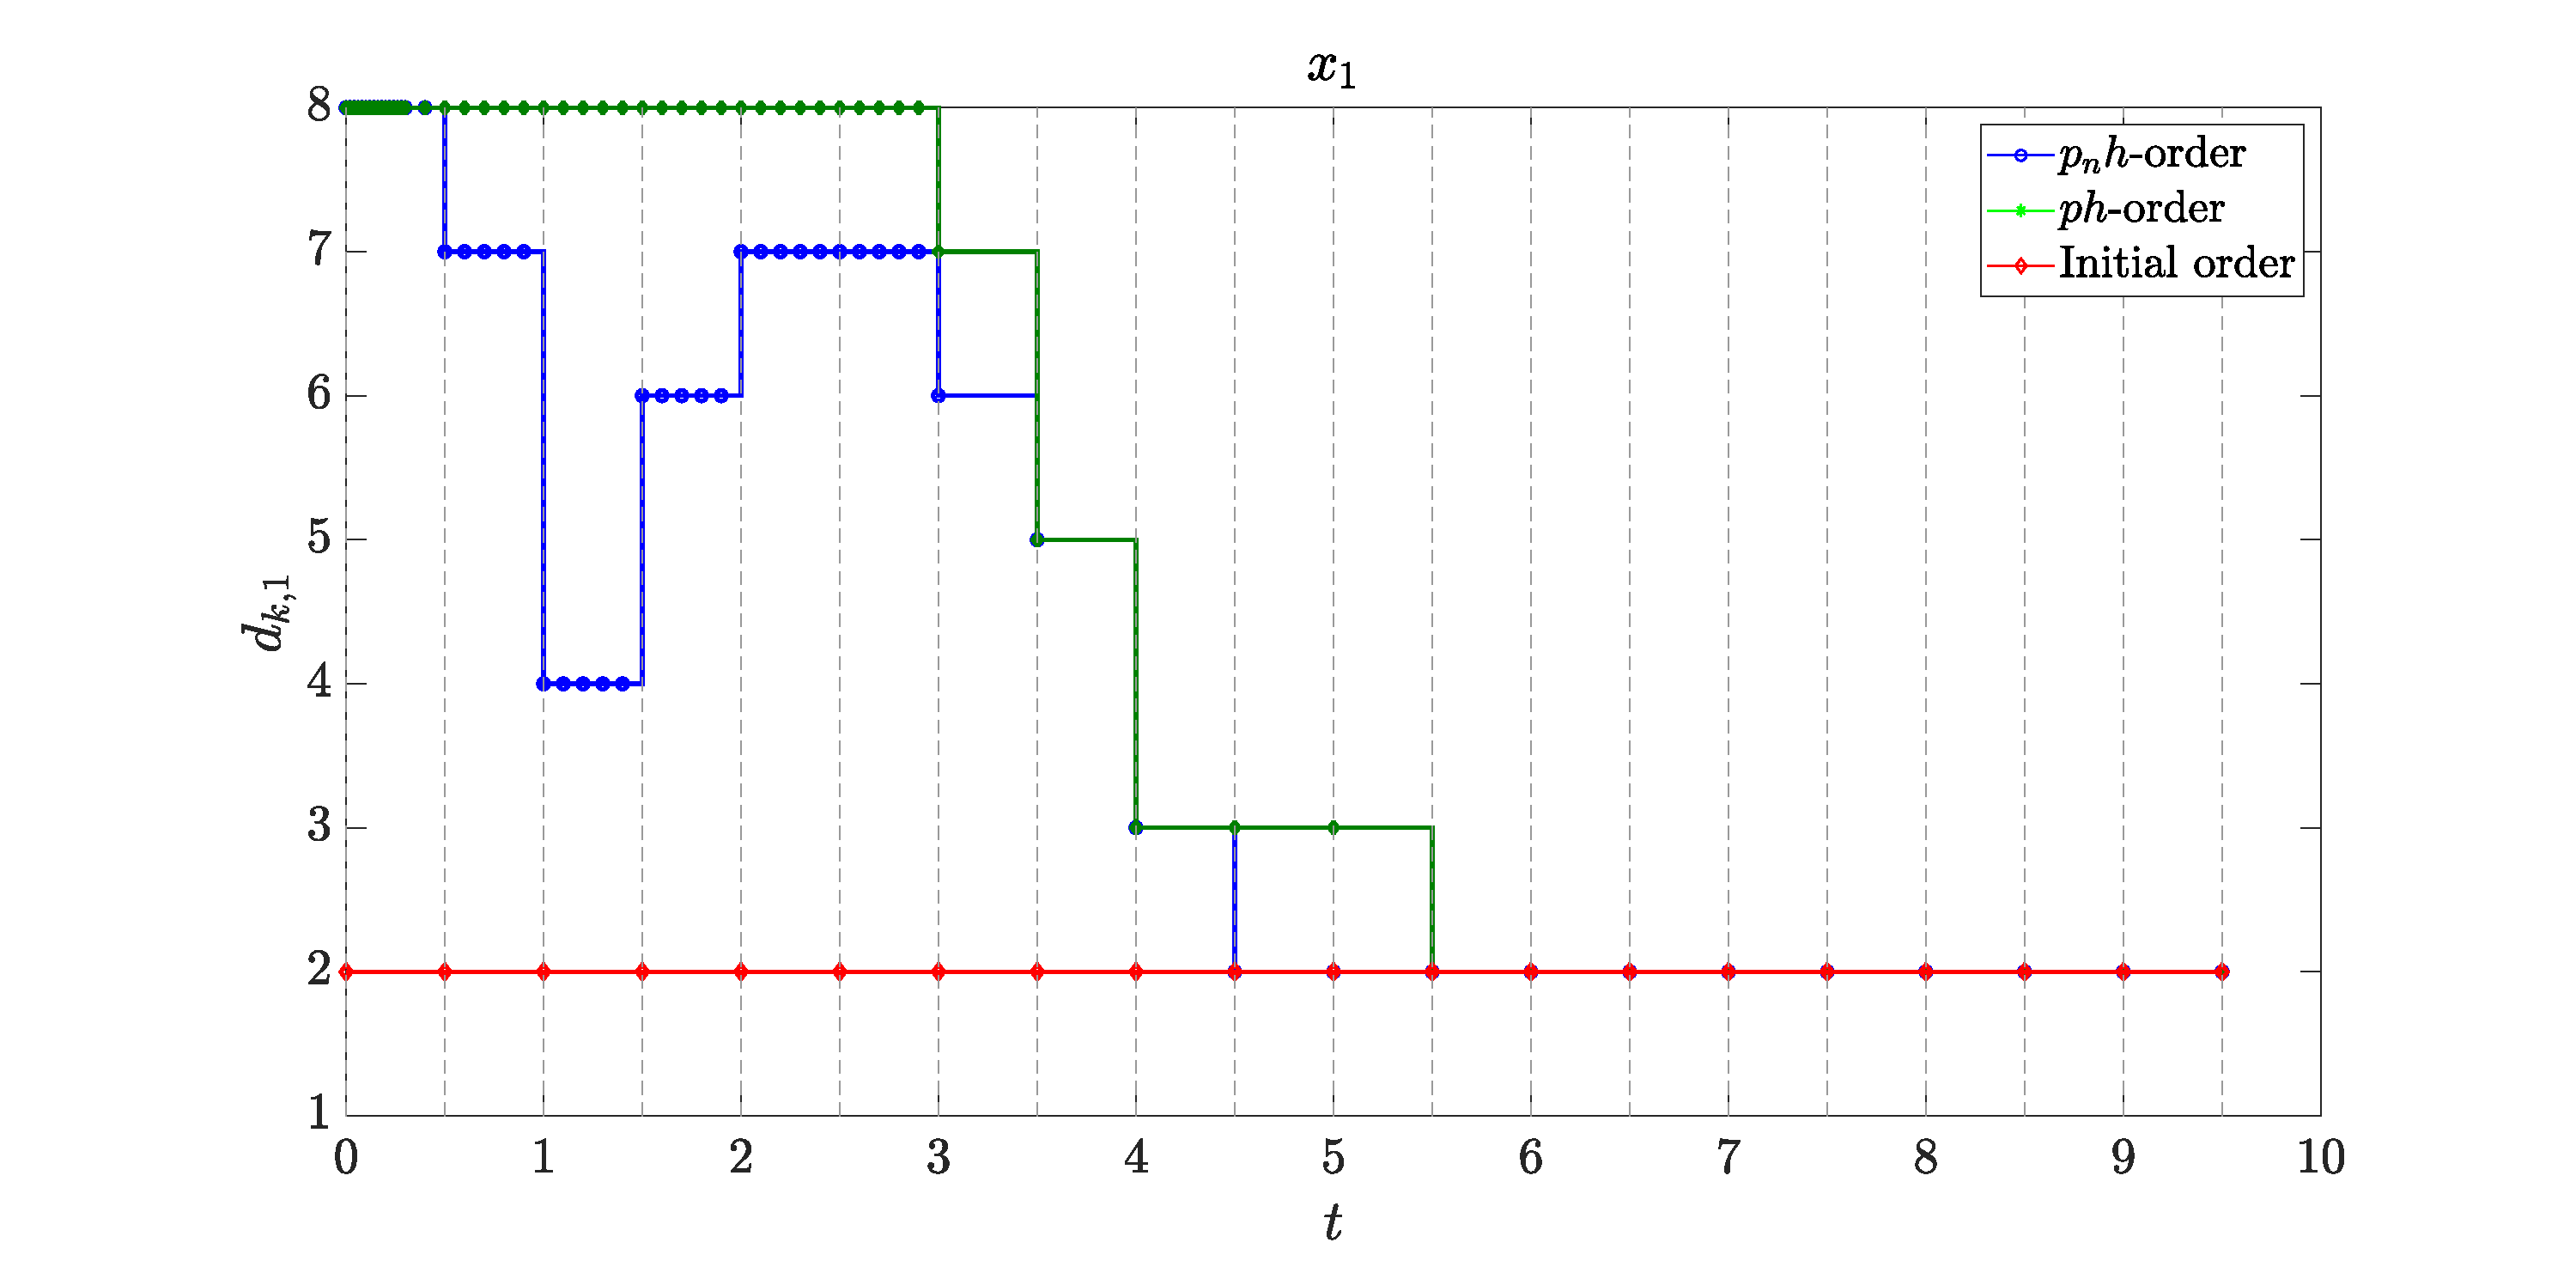
\includegraphics[trim={4cm 0cm 4cm 0cm},clip,width=1.\linewidth]{Img/pnh1_vanderpol}
	\caption{}
	\label{fig:pnhvanderpol}
\end{figure}


%%%%%%%%%%%%%%%%%%%%%%%%%%%%%%%%%%%%%%%%%%%%%%%%%%%%%%%%%%%%%%%%%%%%%%
\subsection*{Rolling Disk}
Esempio disco

%%%%%%%%%%%%%%%%%%%%%%%%%%%%%%%%%%%%%%%%%%%%%%%%%%%%%%%%%%%%%%%%%%%%%%
\subsection*{Free Flying Robot}
Esempio free flying robot

%\cite{latex, goosens} 